\section{Решение}

Фигура строится в два этапа, отрисовка боковых сторон, а также двух оснований, рисуем полигонами по кругу, из трегольников составляя основания, находящиеся на расстоянии H друг от друга, также по окружностям радиуса R.


Ползунком n регулируется точность и мелкость шага отрисовки.

Вместо технологии OpenGl была использована технология WebGl, которая является полной копией первой, только используется для отображения веб графики, для отображения варианта предыдущей лабораторной работы воспользовался технологией, которую поддерживает p5.js

Также для создания анимации используем встроенный счетчик фреймов frameCount, добавим в функцию отрисовки:

$$ y = y * cos (frameCount + y) $$

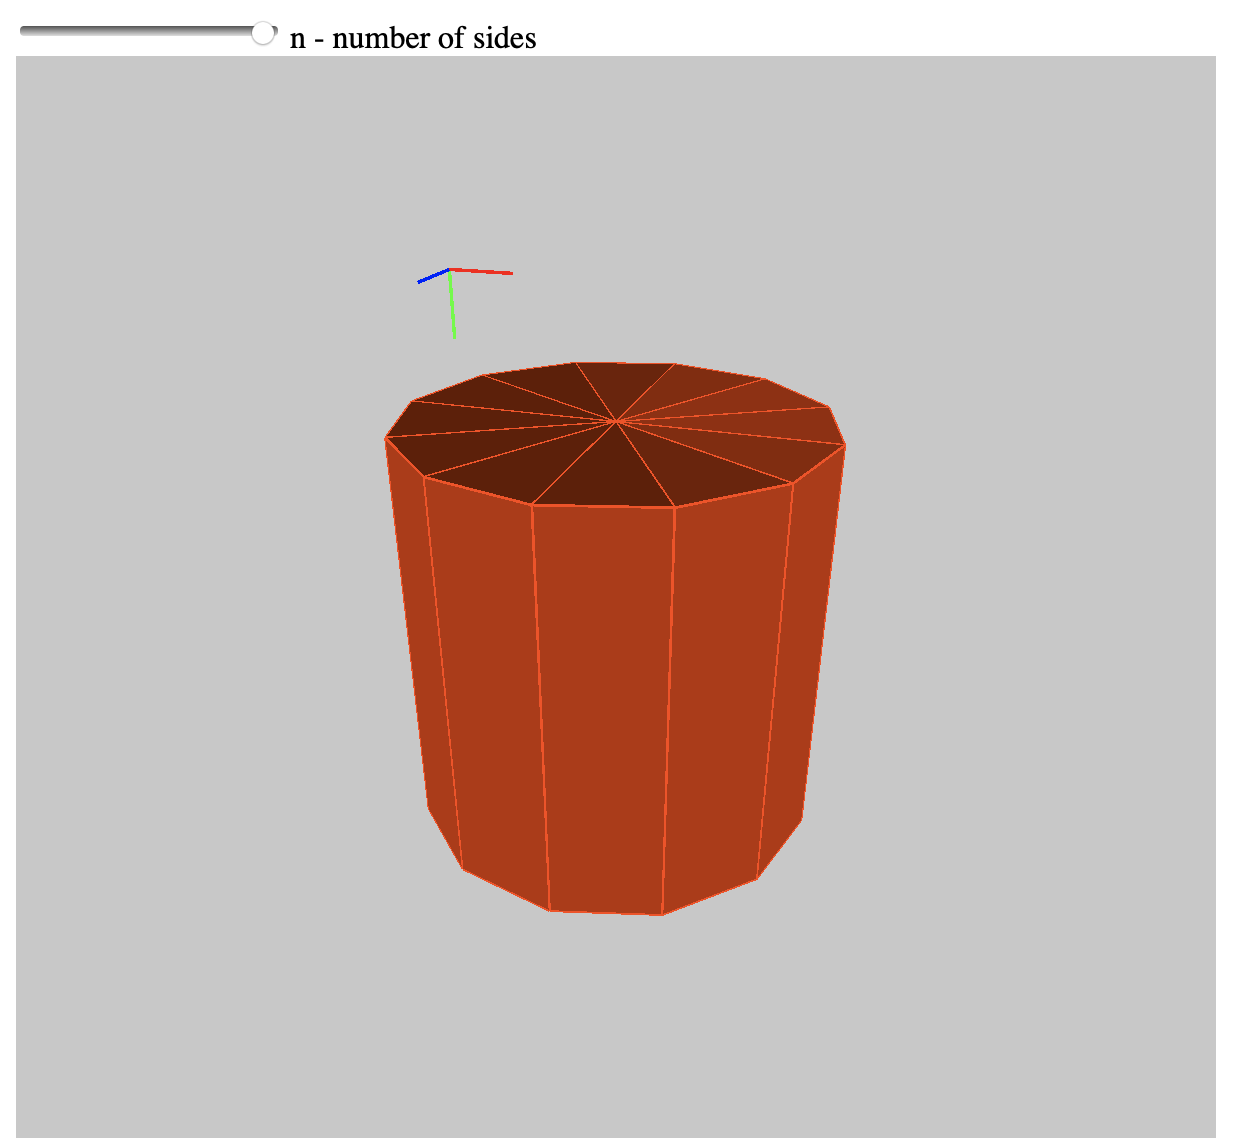
\includegraphics[scale=0.5]{pictures/1.png}

Приведена фугура с малой точностью отрисовки.

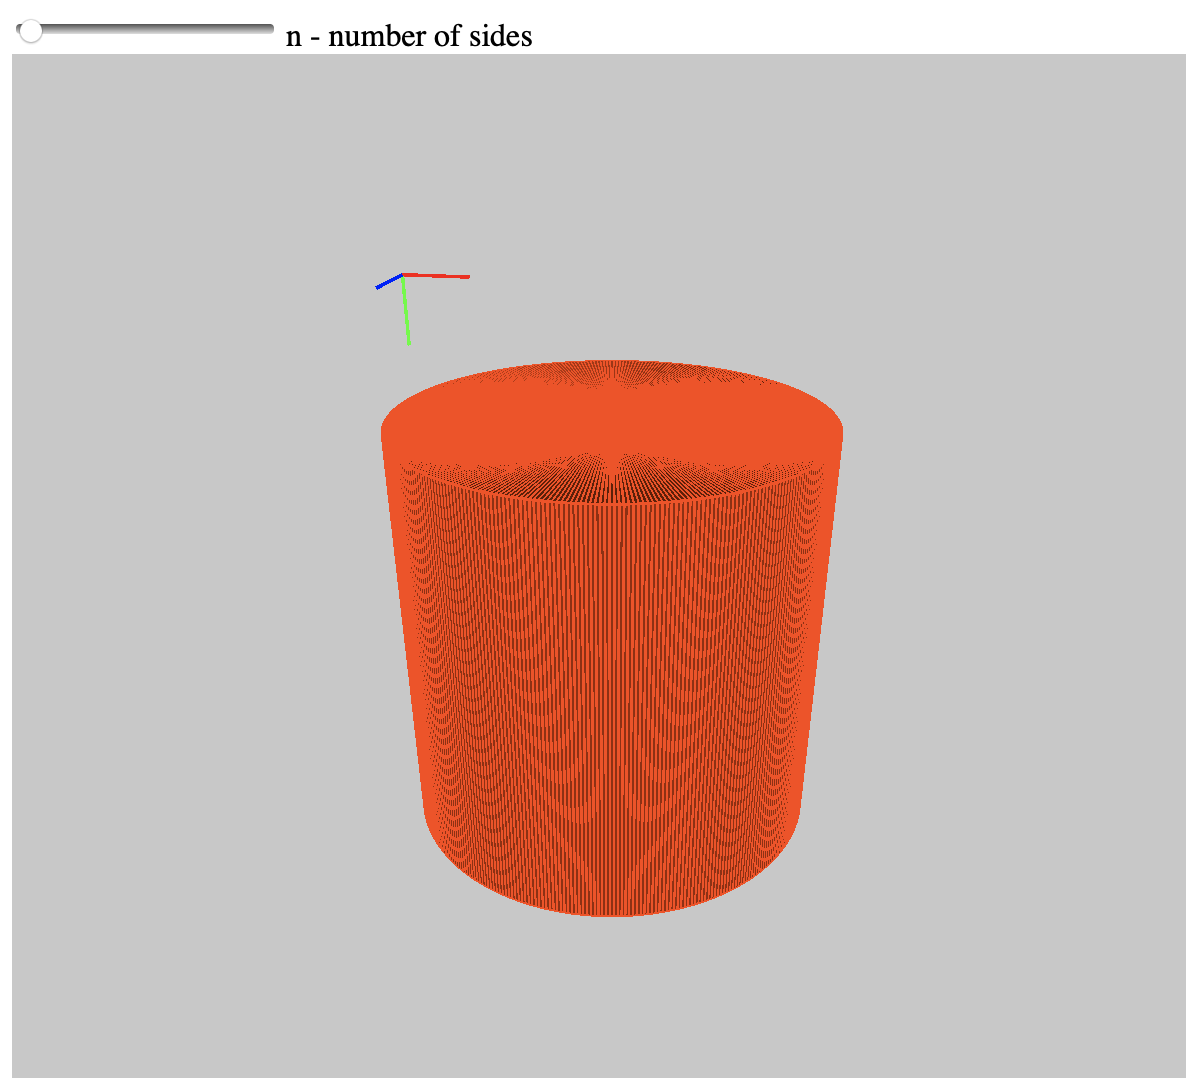
\includegraphics[scale=0.4]{pictures/2.png}

Приведена фугура с высокой точностью отрисовки.

% \section{Исходный код}

% \begin{lstlisting}[language=C++]
% \end{lstlisting}

% \lstset{language=[gnu] make}
% \lstset{
%   language=[gnu] make,
%   keywordstyle=\color{teal}\textbf,
%   stringstyle=\color{blue},
%   identifierstyle=\itshape
% }

% \begin{lstlisting}
% CC = g++
% CCFLAGS = -std=c++14 -Wall -pedantic -O3
% ###____###
% solution : main.cpp *.hpp ; $(CC) $(CCFLAGS) main.cpp -o solution
% clean	 : ;
% \end{lstlisting}

% \section{Консоль}

% \begin{alltt}
% \end{alltt}

% \pagebreak